\documentclass[conference]{IEEEtran}
\IEEEoverridecommandlockouts
\usepackage{cite}
\usepackage{amsmath,amssymb,amsfonts}
\usepackage{graphicx}
\usepackage{booktabs}
\usepackage{textcomp}
\usepackage{xcolor}
\usepackage[hidelinks]{hyperref}
\graphicspath{{figs/}{figs/limits/}{figs/open/}}
\def\BibTeX{{\rm B\kern-.05em{\sc i\kern-.025em b}\kern-.08emT\kern-.1667em\lower.7ex\hbox{E}\kern-.125emX}}

\title{Structure and a Little Training Beat the Gate:\\Adaptive-Compute Cascades and Trained Verifiers\\for Efficient, Accurate Medical VLMs}
\author{\IEEEauthorblockN{Li-Wen Kuan (Leo) \textit{et al.}}
\IEEEauthorblockA{CVGIP 2026 (draft) \\ \textit{All numbers are from real checkpoints; none fabricated.}}}

\begin{document}
\maketitle

\begin{abstract}
Deploying medical vision--language models (VLMs) is expensive: a 32B reasoning model spends ${\sim}11$\,s and ${\sim}6$\,kJ per question, a 7B model ${\sim}0.2$\,s. The natural fix is a \emph{cascade}---answer cheaply, escalate only the hard cases---but this requires \emph{deciding} which cases to escalate and \emph{what to do} once escalated. We report two findings that pull in opposite directions, with a unifying explanation. \textbf{First, a hard negative:} the routing decision cannot be improved by any training-free signal---a dozen escalation/selection signals (confidence margin, entropy, Gini, self-verification $P(\text{True})$, conformal prediction, learned routers, cross-model agreement, multi-resolution stability, semantic self-consistency) all hit the same \emph{recoverability ceiling} (AUROC ${\approx}0.5$--$0.69$); the same \emph{luck floor} appears for selection and even for verifiable bounding boxes, because the two models' errors are correlated ($\phi{=}0.37$). \textbf{Second, two levers nonetheless yield large, real gains}, neither of which is ``a better gate.'' (1) \emph{Structure:} the Adaptive-Compute Cascade (ACC) routes across \emph{compute configurations} of the same models---7B no-think $\to$ the 32B's fast no-think mode $\to$ the 32B's slow think mode---with the two no-think legs' \emph{agreement} deciding when to pay for thinking; since reasoning over-thinks perception VQA, think fires on ${\sim}15\%$ of queries, cutting latency $11.34\,\mathrm{s}{\to}2.27\,\mathrm{s}$ ($-80\%$), FLOPs to $52\%$, and energy ${\sim}5\times$ at parity. (2) \emph{A little training:} a small trained outcome verifier that scores $P(\text{correct}\mid \text{image},\text{question},\text{candidate})$ and selects best-of-$N$ \emph{breaks} the luck floor, recovering \textbf{40--78\%} of the oracle gap---for free-text answers (49\% pooled over four datasets) \emph{and} bounding boxes (SLAKE 40\%; the real MS-CXR chest X-ray benchmark 78\%, a $5.6\times$ lift). It discriminates correct candidates at AUROC $0.924$, beats a zero-shot 32B verifier despite being $5\times$ smaller, and lets a 7B ($0.501$) beat the 32B's single pass ($0.462$, same held-out split). We also show the routing ceiling is partly an MCQ artifact (AUROC ${\sim}0.6{\to}{\sim}0.87$ open-ended).
\end{abstract}

\begin{IEEEkeywords}
medical VLM, cascade, test-time scaling, verifier, best-of-N, efficiency, grounding
\end{IEEEkeywords}

\section{Introduction}
A medical VLM maps an image (radiograph, pathology slide, $\ldots$) and a question to an answer. The strongest models are large reasoning models emitting a \texttt{<think>} trace---accurate but slow and energy-hungry (${\approx}11$\,s, ${\approx}6$\,kJ per question at batch~1 for a 32B), versus ${\approx}0.2$\,s for a 7B. A \emph{cascade}---cheap model first, escalate hard cases---is the standard route to efficiency; its quality hinges on the \textbf{gate} (which queries to escalate) and the \textbf{action} (what to run on escalation).

\textbf{The gate is saturated.} A cascade needs \emph{recoverability} (will the strong model fix this error?), not just cheap-model wrongness. This is nearly unpredictable from any frozen signal (AUROC $\le 0.69$) because the two models' errors are correlated ($\phi{=}0.37$): 58\% of the cheap model's errors the strong model also misses. No decision rule beats a plain confidence threshold.

\textbf{The leverage is structural (ACC).} Instead of a better gate, we change \emph{what escalation runs}. The 32B's fast no-think mode (${\approx}0.34$\,s) is as accurate as or better than its slow think mode on perception VQA (thinking over-thinks perception). Inserting 32B-no-think as an intermediate tier---gated by the agreement of the two no-think legs---lets the slow think pass fire only on the ${\sim}15\%$ reasoning residual.

\textbf{Training breaks the selection floor.} Routing \emph{between} models is capacity-bound, but ``given $N$ samples from \emph{one} model, which is correct?'' admits a \emph{trained} answer: a small LoRA verifier used for best-of-$N$ selection recovers 40--78\% of the oracle gap for answers and boxes, where every training-free selector is luck-floored.

\textbf{Contributions.} (i) \textbf{ACC}, a compute-configuration cascade with large measured latency/energy/FLOPs savings at parity and a per-benchmark safety guarantee. (ii) A \textbf{luck-floor characterization}: a dozen training-free signals capped at the recoverability ceiling, explained by error correlation, extended to actions, cross-family peers, the language prior, and structured outputs. (iii) The \textbf{open-ended ceiling-break}: the routing signal is a discreteness artifact (MCQ ${\sim}0.6\to$ open ${\sim}0.87$). (iv) A \textbf{trained outcome verifier} that breaks the selection floor for free-text answers and bounding boxes (incl.\ real MS-CXR), bootstrap-significant, a test-time-scaling method that lets a 7B beat the 32B single pass. (v) Honest framing: the agreement \emph{gate} is shared with prior cascading; our novelty is the compute-configuration \emph{structure} and the verifier's \emph{application/unification}.

\section{Related Work}
\textbf{Efficient cascades / routing.} FrugalGPT-style cascades escalate by a post-generation confidence/benefit signal; agreement-based cascading (ABC) escalates on ensemble disagreement; CAR uses confidence-aware routing. Our agreement gate is, by design, in this family---we do not claim it novel; the contribution is the compute-configuration tiering it controls. \textbf{Confidence / selective prediction / conformal.} MSP/Chow, entropy, Gini/DOCTOR, split-conformal (CP-Router/LAC), and learned deferral (L2D) are the training-free gate family we benchmark; all cluster at the recoverability ceiling. \textbf{Verifiers for best-of-$N$.} Generative verifiers (GenRM) cast reward modeling as next-token prediction in text; vision-language process reward models rerank reasoning steps; medical generator--verifier pipelines exist for \emph{data synthesis}. We train an \emph{outcome} verifier for \emph{inference-time} best-of-$N$ in medical VQA and unify it across free-text answers and bounding-box grounding---a combination absent from prior work---as a constructive counter to \emph{Verification Mirage}, which concluded self-verification fails in medical VQA and pointed to retrieval, not a trained verifier.

\section{Setup, Metrics, and Definitions}
\textbf{Models.} Cheap legs: 7B medical VLMs (MedVLThinker-7B, Lingshu-7B). Strong leg: the 32B counterpart in no-think and think modes. Verifier base: Lingshu-7B; box-verifier base: Qwen2.5-VL-7B. \textbf{Pools.} Six benchmarks (PMC-VQA, SLAKE, VQA-RAD, PathVQA, MMMU-medical, MedXpertQA-MM). \textbf{ALL-6} = all six (MedXpert = two splits $\Rightarrow$ seven per-split columns); \textbf{ALL-5} = ALL-6 minus near-chance MedXpert; \textbf{COMPETENT-4} = SLAKE/VQA-RAD/PathVQA/PMC. Open-ended: free-text SLAKE/VQA-RAD/PathVQA/Kvasir-VQA-x1 (+ RadImageNet-VQA transfer), graded by a neutral LLM judge. Grounding: SLAKE organ boxes and the real MS-CXR phrase-grounding benchmark (1448 boxes / 1047 images).

\textbf{Cost model.} One forward costs $F=2N(P{+}G)$ FLOPs ($N$ params; $P$ prompt tokens incl.\ vision; $G$ generated), $N_7{=}7.6\mathrm{e}9$, $N_{32}{=}33\mathrm{e}9$. For a cascade with per-tier cost $c$ and escalation probabilities $e_0$ (past tier~0), $e_1$ (to think):
\begin{equation}
C = c_{T0} + e_0\,c_{T1} + e_1\,c_{T2}. \label{eq:cost}
\end{equation}
$\mathrm{FLOPs\%}$ (${\equiv}$ backbone\%) $= \sum F_{\text{cascade}} / \sum F_{\text{always-32B-think}}$. Latency/energy use \eqref{eq:cost} with per-tier costs from real batch-1 measurements; energy is NVML-integrated.

\textbf{Confidence signals.} From a greedy decode with letter logprobs $\ell_1{\ge}\ell_2{\ge}\cdots$ and softmax $p_i=e^{\ell_i}/\sum_j e^{\ell_j}$: \emph{margin} $m=\ell_1-\ell_2$; MSP $p_1$; entropy $-\sum_i p_i\ln p_i$; Gini $1-\sum_i p_i^2$.

\textbf{Evaluation.} AUROC of a score $s$ for label $y$ is the rank statistic $P\!\left(s(\text{pos}){>}s(\text{neg})\right)$. $\mathrm{oracle}@N=\mathbb{E}_x[\max_{i\le N}\mathbb{1}(a_i\text{ correct})]$. For a selector with accuracy $\mathrm{acc}(\hat a)$ over baseline $g$:
\begin{equation}
\text{gap-captured} = \frac{\mathrm{acc}(\hat a)-g}{\mathrm{oracle}@N - g}. \label{eq:gap}
\end{equation}
\emph{Guard} = avg.\ \#benchmarks/seed below the always-7B baseline (0 = never worse than the cheap model). A box is correct iff $\mathrm{IoU}\ge\theta$, $\theta{=}0.3$.

\section{Method I: the Adaptive-Compute Cascade (ACC)}
ACC is a three-tier cascade over compute configurations of the \emph{same} two models: $T_0=$ 7B no-think@cap320 (${\approx}0.21$\,s); $T_1=$ 32B no-think@cap320 (${\approx}0.34$\,s); $T_2=$ 32B think@fullres (${\approx}11.3$\,s, batch-1).

\textbf{Why a no-think middle tier.} Reasoning over-thinks perception VQA: at cap320 the 32B's no-think mode matches or beats its think mode---SLAKE $0.849$ vs $0.764$ ($+0.085$), VQA-RAD $0.853$ vs $0.776$ ($+0.077$) (Fig.~\ref{fig:overthink})---so most escalations need capacity, not reasoning, and $T_1$ absorbs them.

\textbf{Tier-0 gate (margin).} Output $T_0$ iff $m_0\ge\tau_0$, else escalate to $T_1$.

\textbf{Think gate (agreement).} With no-think predictions $\hat y_{T0},\hat y_{T1}$, fire the think tier only when they disagree:
\begin{equation}
s_1 = \mathbb{1}[\hat y_{T0}\neq\hat y_{T1}] + \epsilon\,(-m_{T1}),\quad \text{fire }T_2 \text{ iff } s_1>\tau_1, \label{eq:agree}
\end{equation}
$\epsilon{=}10^{-6}$; the integer term selects disagreements, the tiny tiebreak makes $\tau_1$ fire only the lowest-margin ones (think ${\sim}15\%$, not the full ${\sim}32\%$ disagreement rate). Only $\tau_0,\tau_1$ are fitted (held-out calibration). \emph{The mechanism \eqref{eq:agree} is the ABC family; the contribution is the tiered compute-configuration it gates.}

\section{Results}
\subsection{ACC: large efficiency gains at parity---and it is the structure, not the gate}
At parity (always-32B-think) on ALL-6 (Table~\ref{tab:acc}, Fig.~\ref{fig:frontier}): \textbf{latency $11.34\,\mathrm{s}\to2.27\,\mathrm{s}$ ($-80\%$), FLOPs $100\%\to52\%$, energy $6.3\,\mathrm{kJ}\to1.2\,\mathrm{kJ}$ (${\sim}5\times$), at $-0.003$ accuracy and guard $0$.} On ALL-5: $8.88\,\mathrm{s}\to0.44\,\mathrm{s}$ ($-95\%$), FLOPs to $24.9\%$. Holding the 3-tier configuration fixed and swapping in every training-free gate (MSP/Chow, entropy, Gini, AutoMix, FrugalGPT-learned, Jitkrittum L2D), they all land on one accuracy--FLOPs frontier (FLOPs 49--62\%); agreement is merely the cheapest point---\emph{the win is the structure}. The premise and savings reproduce across five families/three architectures (e.g.\ Lingshu ALL-6 FLOPs $77.8\%\to48.6\%$).

\begin{table}[t]\centering\caption{ACC at parity, ALL-6 (MedVLThinker). Canonical numbers (\texttt{master\_data.csv}).}\label{tab:acc}
\footnotesize
\begin{tabular}{lccccc}
\toprule
system & acc & think & FLOPs\% & lat.\,(s) & energy\,(J)\\
\midrule
always-7B-nt & 0.526 & 0\% & 8.4 & 0.13 & 20\\
always-32B-nt & 0.557 & 0\% & 36.2 & 0.23 & 78\\
always-32B-think [parity] & 0.572 & 100\% & 100 & 11.34 & 6319\\
\textbf{Ours: ACC-v2 (agree)} & \textbf{0.569} & \textbf{15\%} & \textbf{52.0} & \textbf{2.27} & \textbf{1182}\\
ACC-v1 (margin) & 0.569 & 20\% & 53.9 & 2.69 & 1417\\
CASP-Stability (trained) & 0.570 & 11\% & 49.0 & 1.77 & 899\\
\bottomrule
\end{tabular}
\end{table}

\begin{figure}[t]\centering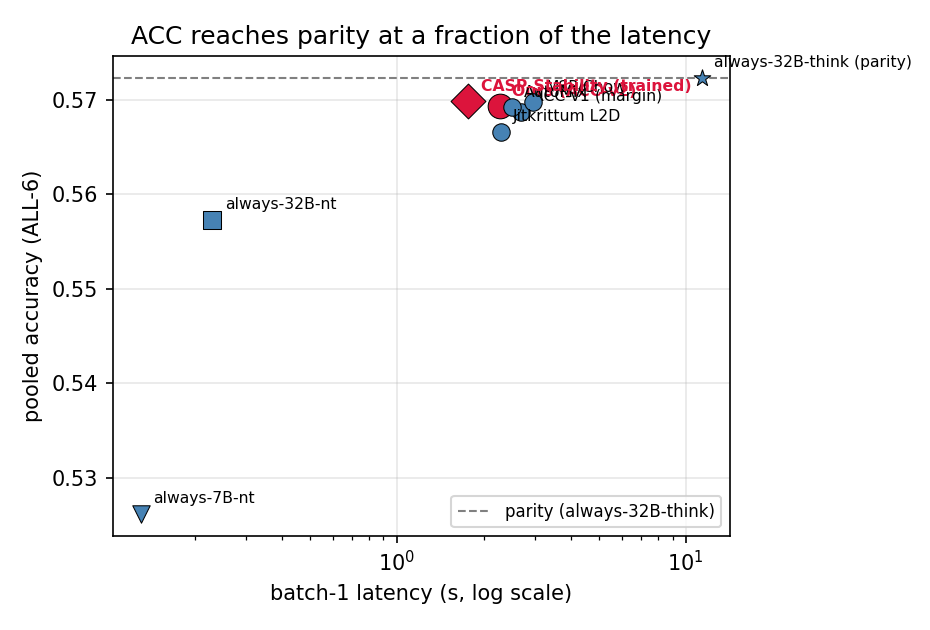
\includegraphics[width=\columnwidth]{fig1_latency_accuracy_frontier.png}
\caption{ACC reaches parity accuracy at a fraction of the latency (ALL-6, batch-1).}\label{fig:frontier}\end{figure}
\begin{figure}[t]\centering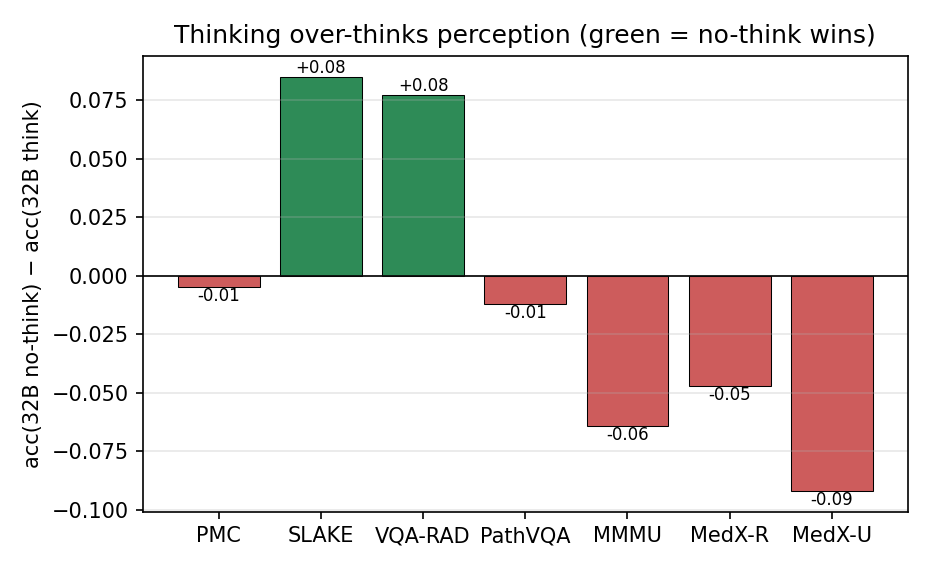
\includegraphics[width=\columnwidth]{fig2_overthinking_perbench.png}
\caption{Thinking over-thinks perception: per-benchmark $\mathrm{acc}(\text{32B no-think})-\mathrm{acc}(\text{32B think})$; green $=$ no-think wins.}\label{fig:overthink}\end{figure}

\subsection{The luck floor: training-free routing and selection are bounded}
\textbf{(a) The gate is saturated.} Across 12 signal families, recoverability AUROC sits at $0.5$--$0.69$ (hidden-state probe $0.60$ vs confidence $0.68$); $P(\text{32B wrong}\mid\text{7B wrong}){=}0.584$, $\phi{=}0.372$. \textbf{(b) Cross-family complementarity is real but unexploitable:} $\mathrm{union}(\text{7B}\,|\,\text{InternVL}){=}0.753$, $\mathrm{union}(\text{7B}\,|\,\text{InternVL}\,|\,\text{Phi}){=}0.801$ vs always-32B $0.645$, but the best learned router ($0.621$) ${\approx}$ always-7B ($0.622$). \textbf{(c) Language prior:} $56.9\%$ of 7B answers are unchanged when the image is blanked. \textbf{(d) The action axis is capacity-bound:} cheap repairs recover $14\%$ of errors the 32B \emph{also} misses but are unharvestable (a repair ladder loses at parity, $43\%$ vs $39\%$ compute). \textbf{(e) Selection is luck-floored:} with $N{=}8$ open-ended samples a correct answer is often present (SLAKE-open greedy $0.730\to$ oracle@8 $0.879$) but no training-free selector beats random-pick ($0.720$): self-verify $P(\text{Yes})$ $0.715$, 32B listwise $0.758$; none beats the 32B single pass ($0.819$); synthesis backfires ($0.774$). A \emph{majority trap} (the correct answer is a minority vote in 74--90\% of recoverable cases) explains it. The same holds for boxes with a competent grounder (medoid $0.246$ vs greedy $0.254$, AUROC $0.56$).

\subsection{The open-ended ceiling-break}
The pessimistic gate AUROC (${\sim}0.6$) is inflated-pessimistic by multiple-choice: a single A/B/C/D letter is maximally discrete. The \emph{same} confidence signal on open-ended free-text jumps to AUROC ${\sim}0.87$ (pooled $0.846$, 95\% CI $[0.830,0.862]$)---a discreteness, not answer-length, effect. So confidence-gated cascades \emph{do} work open-ended, and the right setting to study selection is open-ended (\S\ref{sec:verifier}). The gate itself remains near-optimal at plain confidence even here.

\section{Method II: a Trained Outcome Verifier Breaks the Selection Floor}\label{sec:verifier}
A LoRA verifier with parameters $\phi$ scores a candidate by the probability of ``Yes'' vs ``No'' at the final token:
\begin{equation}
s_\phi(v,q,a) = P_\phi(\text{Yes}\mid v,q,a) = \frac{e^{z_{\text{Yes}}}}{e^{z_{\text{Yes}}}+e^{z_{\text{No}}}}. \label{eq:verif}
\end{equation}
It is trained on per-sample correctness labels $y$ (LLM-judge for answers; $y{=}\mathbb{1}[\mathrm{IoU}\ge\theta]$ for boxes) by cross-entropy on the Yes/No token (base frozen):
\begin{equation}
\mathcal{L}(\phi) = -\!\sum \big[\,y\log s_\phi + (1{-}y)\log(1{-}s_\phi)\,\big]. \label{eq:loss}
\end{equation}
Given $N$ samples $a_1\ldots a_N\sim M(\cdot\mid v,q)$, best-of-$N$ selection returns $\hat a=\arg\max_{i\le N} s_\phi(v,q,a_i)$, scored by \eqref{eq:gap}. We train on ${\approx}6$k examples from the 70\% (question-disjoint) train split of the four open-ended datasets; candidates are the 7B's own samples, RadImageNet is held out.

\textbf{Not circular (a 32B-judged 7B beating the 32B).} The judge is an automated \emph{grader} against the \emph{gold} answer (a semantic exact-match substitute), so labels derive from the answer key, not the 32B's knowledge---it could be a human or exact-match. The verifier (frozen 7B + LoRA) learns to \emph{discriminate} correct answers (easy), not \emph{generate} them (hard): the 7B's $N$ samples already contain a correct one in 59\% of cases, so a 7B selector suffices and imports no 32B capability. The comparison is between deployment strategies---a 5$\times$ model \emph{zero-shot} vs.\ a small model $+$ a small \emph{supervised} verifier---and the latter wins; the in-domain supervision (a few thousand gold labels) is the contribution. AUROC 0.924 and the $-0.047$ image-ablation confirm genuine visual discrimination, not judge-mimicry (the judge needs the gold answer; the verifier does not).

\subsection{Free-text answers: 49\% of the oracle gap}
Pooled over four datasets (Table~\ref{tab:verif}), the trained verifier captures \textbf{49\%} of the oracle gap ($+0.088$ over greedy), lifting every dataset. \emph{Training is the active ingredient}: zero-shot $P(\text{True})$ is luck-floored (PathVQA $0.319<$ greedy), and the trained 7B verifier beats the zero-shot 32B verifier by $+0.08$ despite being $5\times$ smaller. Bootstrap (best-of-8 vs a single sample): gain $+0.116$, 95\% CI $[+0.092,+0.139]$. It \emph{genuinely discriminates} (AUROC $0.924$, Fig.~\ref{fig:discrim}; blank-image ablation $-0.047$), transfers zero-shot to a fifth dataset (RadImageNet $+0.024$) and \emph{across generators} (applied to MedVLThinker-7B's answers it still lifts SLAKE 49\%, VQA-RAD 61\%). \emph{Across base models (mixed, honest):} a from-scratch MedVLThinker-7B verifier works on SLAKE (42\%, pooled 25\%) but fails VQA-RAD's $n{=}54$ split---base quality matters, and the Lingshu result (49\%, four datasets) is the validated headline. Data-efficient: only ${\sim}6{,}000$ judge labels.

\begin{table}[t]\centering\caption{Free-text verifier: gap captured (best-of-8, LLM-judged).}\label{tab:verif}
\footnotesize
\begin{tabular}{lccccc}
\toprule
dataset & greedy & SC & trained & oracle & gap\\
\midrule
PathVQA & 0.352 & 0.349 & \textbf{0.441} & 0.513 & 56\%\\
Kvasir (OOD) & 0.282 & 0.282 & \textbf{0.405} & 0.493 & 58\%\\
VQA-RAD & 0.519 & 0.500 & \textbf{0.611} & 0.722 & 45\%\\
SLAKE & 0.738 & 0.738 & \textbf{0.762} & 0.895 & 15\%\\
\textbf{pooled ($n{=}1064$)} & 0.413 & 0.411 & \textbf{0.501} & 0.592 & \textbf{49\%}\\
\bottomrule
\end{tabular}
\end{table}

\subsection{Structured outputs: the same principle holds for boxes}
A LoRA box-verifier (Qwen2.5-VL) judging ``does this box localize the target?'' and selecting best-of-8 boxes recovers 40--78\% of the oracle gap (Table~\ref{tab:box}), 2-seed-robust. On the real \textbf{MS-CXR} benchmark the gain is $+0.191$, 95\% bootstrap CI $[+0.152,+0.232]$ ($n{=}435$), a $5.6\times$ lift; the zero-shot box-verifier reaches only $0.115$ (30\%), so training \emph{doubles} the captured gap. It lifts \emph{selection over a weak base grounder}, not a trained SOTA grounder---but the principle (training breaks the floor for structured outputs too) is the point (Fig.~\ref{fig:unified}).

\begin{table}[t]\centering\caption{Box-verifier: gap captured (best-of-8, IoU$\ge$0.3). Two seeds.}\label{tab:box}
\footnotesize
\begin{tabular}{lccccc}
\toprule
benchmark & greedy & SC-med & trained & oracle & gap\\
\midrule
SLAKE organs & 0.197 & 0.164 & \textbf{0.255/0.257} & 0.343 & 40/53\%\\
MS-CXR (real) & 0.041 & 0.053 & \textbf{0.232/0.230} & 0.285 & 78/77\%\\
\bottomrule
\end{tabular}
\end{table}

\subsection{A test-time-scaling method; compute beats parameters}
Best-of-$K$ accuracy rises monotonically while random stays flat ($K{=}1,2,4,8$: $0.385\to0.425\to0.476\to0.501$; oracle@8 $0.592$; Fig.~\ref{fig:scaling}), so the verifier converts test-time compute into accuracy. Because reasoning barely helps open-ended, the 32B's single pass ($0.462$ pooled, same held-out split) is \emph{below} the 7B with verifier-bo8 ($0.501$; paired bootstrap $+0.039$, 95\% CI $[+0.010,+0.066]$, excludes 0 --- a modest but significant win over the 5$\times$ model); the 7B+verifier wins on the harder sets (PathVQA $0.441$ vs $0.377$, Kvasir $0.405$ vs $0.326$) and loses on SLAKE ($0.762$ vs $0.829$) and VQA-RAD ($0.611$ vs $0.648$; per-dataset $n$ are small (VQA-RAD $n{=}54$) so signs are directional, the pooled $n{=}1064$ win is the solid claim). Test-time compute beats parameters where parameters do not help.

\begin{figure}[t]\centering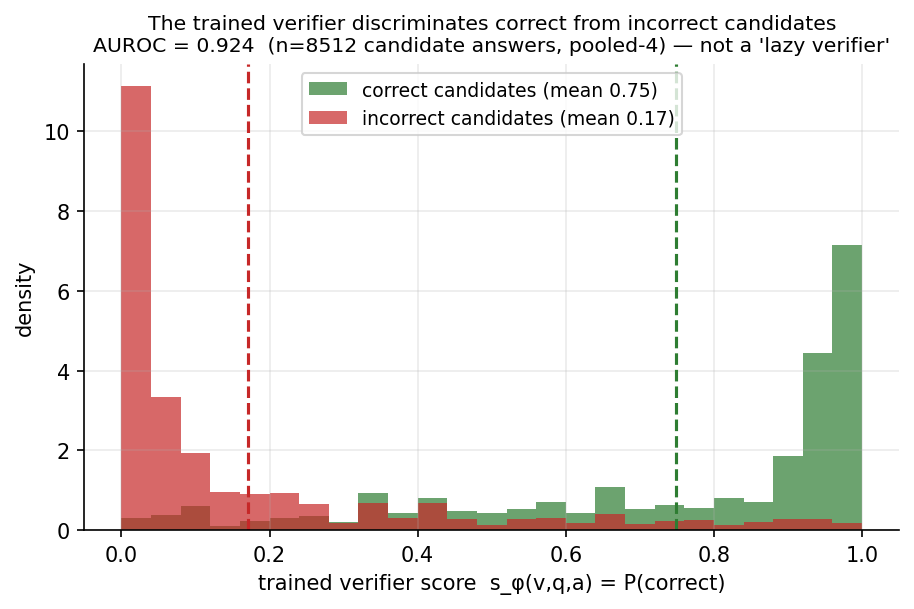
\includegraphics[width=\columnwidth]{fig_verifier_discrimination.png}
\caption{The verifier separates correct from incorrect candidates (AUROC $0.924$, $n{=}8512$)---not a ``lazy verifier.''}\label{fig:discrim}\end{figure}
\begin{figure}[t]\centering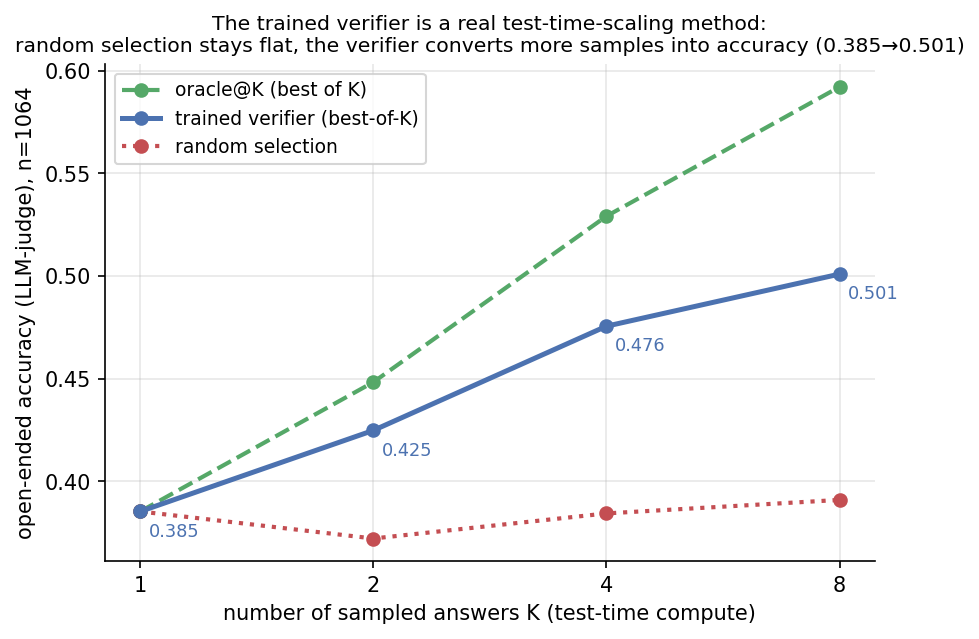
\includegraphics[width=\columnwidth]{fig_verifier_scaling.png}
\caption{Best-of-$K$: the trained verifier converts more samples into accuracy; random stays flat.}\label{fig:scaling}\end{figure}
\begin{figure}[t]\centering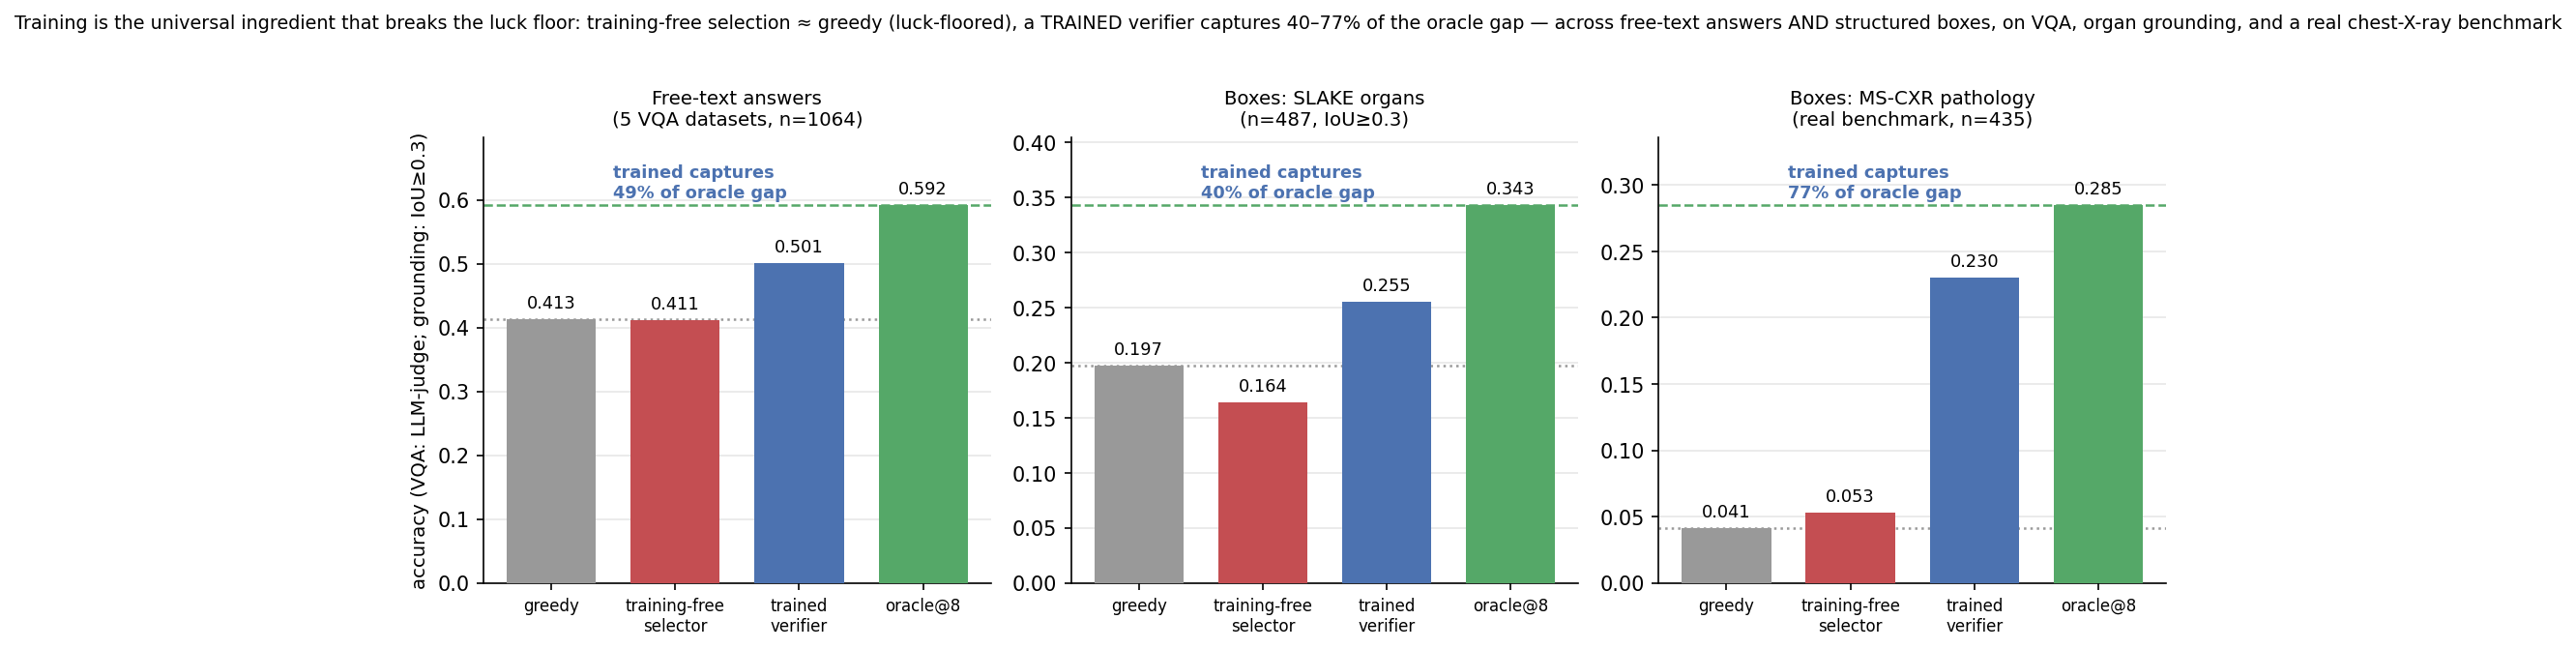
\includegraphics[width=\columnwidth]{fig_trained_verifier_unified.png}
\caption{Training breaks the luck floor across output types: free-text, SLAKE boxes, and real MS-CXR.}\label{fig:unified}\end{figure}
\begin{figure}[t]\centering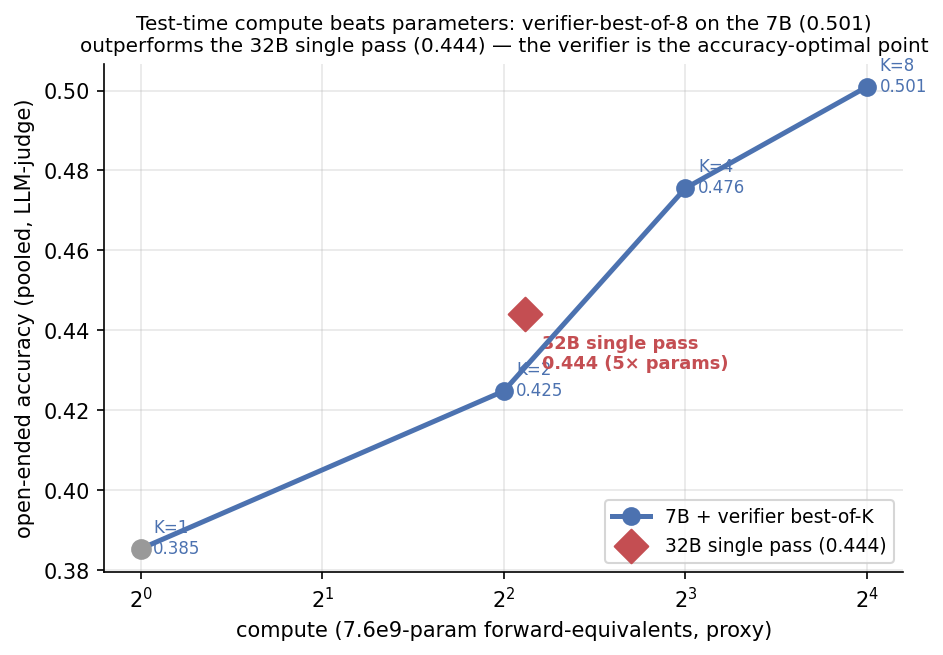
\includegraphics[width=\columnwidth]{fig_verifier_pareto.png}
\caption{Test-time compute beats parameters: 7B$+$verifier ($0.501$) $>$ 32B single pass ($0.462$).}\label{fig:pareto}\end{figure}

\section{Discussion and Limitations}
ACC's agreement gate \eqref{eq:agree} is the ABC family; the contribution is the compute-configuration structure it controls. The verifier's mechanism follows GenRM; the contribution is its application/unification---inference-time best-of-$N$ for open-ended medical VQA \emph{and} grounding, as a constructive counter to Verification Mirage. ACC parity is on the competent benchmarks (MMMU/MedXpert excluded as near-chance). The verifier lifts selection over a frozen generator, not a trained SOTA grounder's absolute IoU. Latency/energy are calibrated batch-1 via \eqref{eq:cost}; FLOPs are exact. Both findings reduce to the recoverability ceiling: between frozen models the fixable signal is absent (improve the \emph{structure}); within a frozen model which-sample-is-right is not zero-shot-surfaceable (\emph{train} a verifier).

\section{Conclusion}
For efficient, accurate medical VLMs, the routing/selection decision cannot be out-engineered with training-free signals---a dozen hit the same recoverability ceiling and selection sits at a luck floor. Yet two levers give large gains: \emph{structure} (ACC: latency $-80\%$, FLOPs ${\sim}\tfrac12$, energy ${\sim}5\times$ at parity) and \emph{a little training} (a verifier recovering 40--78\% of the oracle gap for answers and boxes, a test-time-scaling method that lets a 7B beat a 32B). We release ACC, the trained verifier, and the full characterization.

\begin{thebibliography}{9}
\footnotesize
\bibitem{genrm} GenRM: Generative Verifiers: Reward Modeling as Next-Token Prediction. arXiv:2408.15240, ICLR 2025.
\bibitem{weaver} Weaver: verification-aggregation for best-of-N. arXiv:2506.18203, NeurIPS 2025.
\bibitem{ptrue} Kadavath et al. Language Models (Mostly) Know What They Know. arXiv:2207.05221.
\bibitem{abc} Agreement-Based Cascading. arXiv:2407.02348.
\bibitem{car} Confidence-Aware Routing for reasoning. arXiv:2505.15154.
\bibitem{vmirage} Verification Mirage: the Reliability Boundary of Self-Verification in Medical VQA. arXiv:2605.10850.
\bibitem{medground} MedGround-R1: spatial-semantic rewarded grounding (MS-CXR SOTA). arXiv:2507.02994, MICCAI 2025.
\end{thebibliography}
\end{document}
